\chapter{Conclusioni}

\section{Sviluppi futuri}
L'applicazione realizzata ha voluto includere le funzionalità essenziali per poter essere di supporto durante la competizione. Alcune funzionalità sono state aggiunte per poter aumentare la flessibilità dell'applicazione, in modo che possa adattarsi in base alle esigenze: ad esempio, la possibilità di determinare ogni quanti secondi effettuare una connessione al server per ricevere i dati. Inoltre è stata realizzata una grafica ordinata e pulita, in modo da poter individuare immediatamente i dati necessari. Oltre agli aspetti visivi, la gran parte del lavoro è stato fatto nel \textit{background}, ovvero, nella strutturazione di un'architettura che fosse solida e flessibile per poter supportare in futuro delle nuove funzionalità. Pertanto in questa sezione si introducono dei possibili sviluppi futuri, di cui alcuni sono già stati impostati.

\subsection{Notifiche push}
Le \textit{notifiche push} sono una funzionalità peculiare dei dispositivi mobili. Nel contesto d'uso, le notifiche push potrebbero essere utili nel caso in cui si volesse attirare l'attenzione dell'utente per segnalare un determinato evento. Si assuma di trovarsi nel caso in cui l'utente stia monitorando un certo set di dati da una determinata schermata. Se l'applicazione inviasse una notifica push per segnalare, ad esempio, un aumento improvviso della velocità apparente del vento, l'utente se ne accorgerebbe e potrebbe andare nell'apposita schermata per analizzare il dato e verificare se l'avviso ricevuto può essere considerato rilevante o meno.

L'utilizzo delle notifiche push potrebbe essere esteso anche per altre funzionalità in quanto è uno strumento molto flessibile e molto utile.

\begin{figure}[htp]
	\centering
	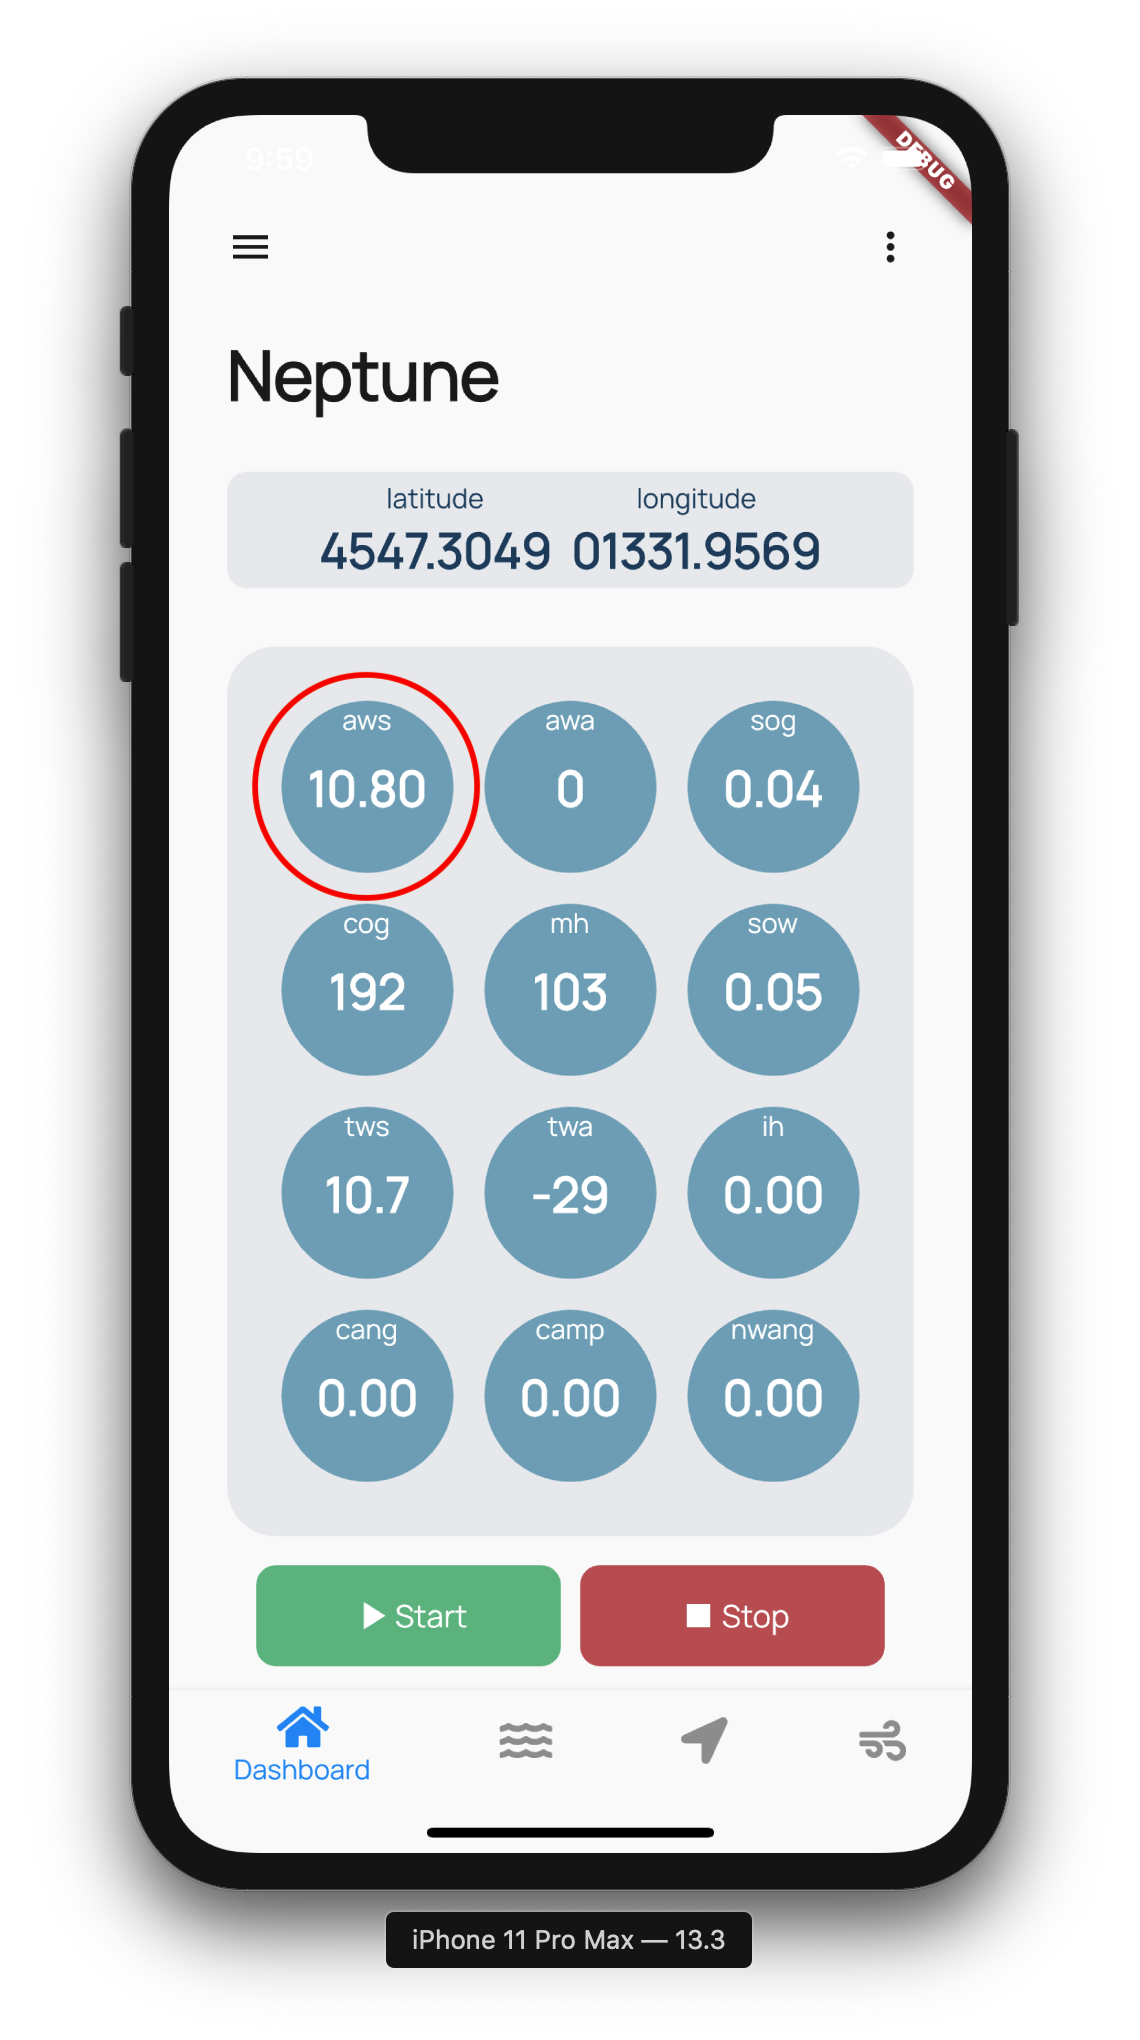
\includegraphics[scale=0.25]{dashboard_tap}
	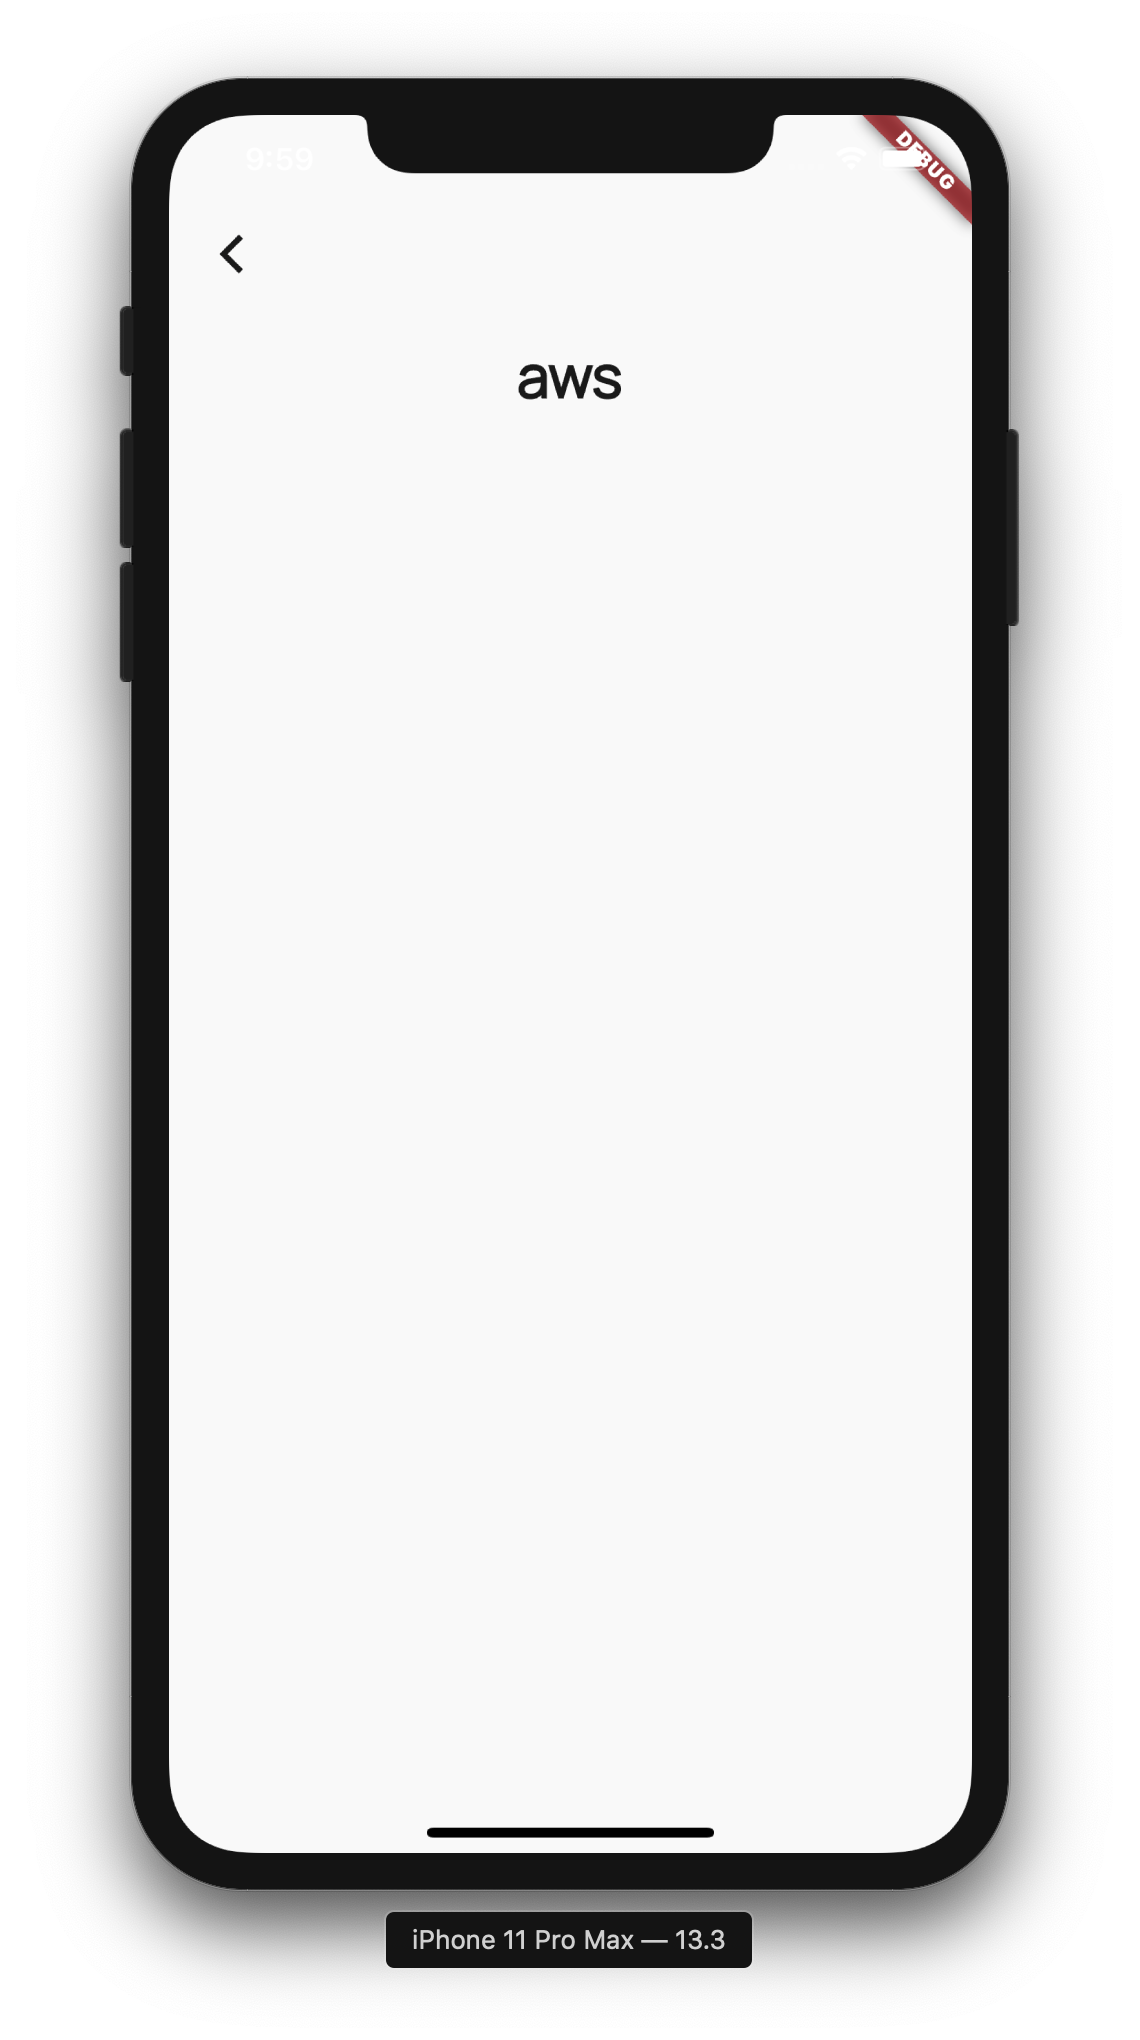
\includegraphics[scale=0.25]{dashboard_detail}
	\caption[Sviluppi futuri - Dashboard]{Facendo tap sul dato \textit{aws}, si aprirà la schermata di destra.}\label{xyz}
\end{figure}

\begin{figure}[htp]
	\centering
	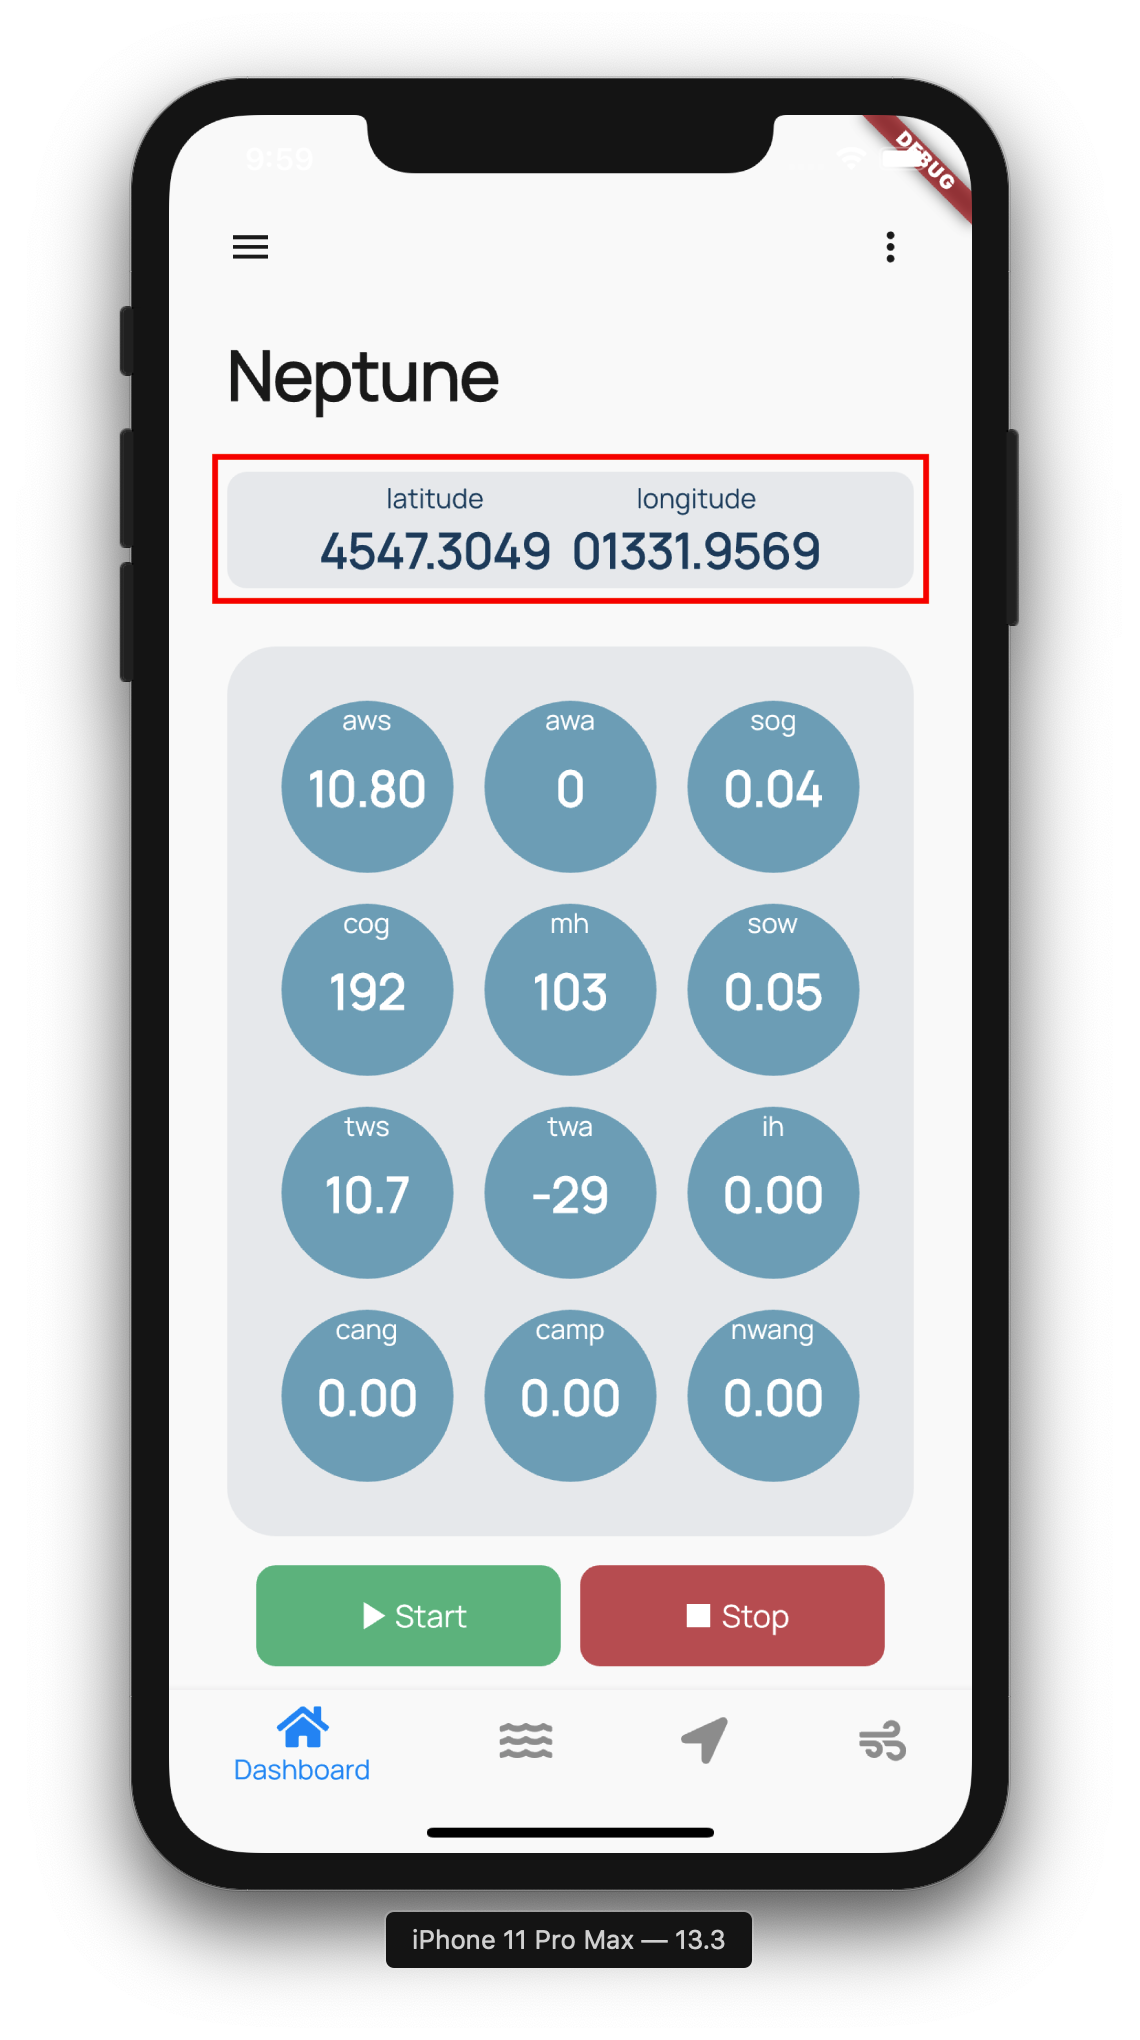
\includegraphics[scale=0.25]{location_tap}
	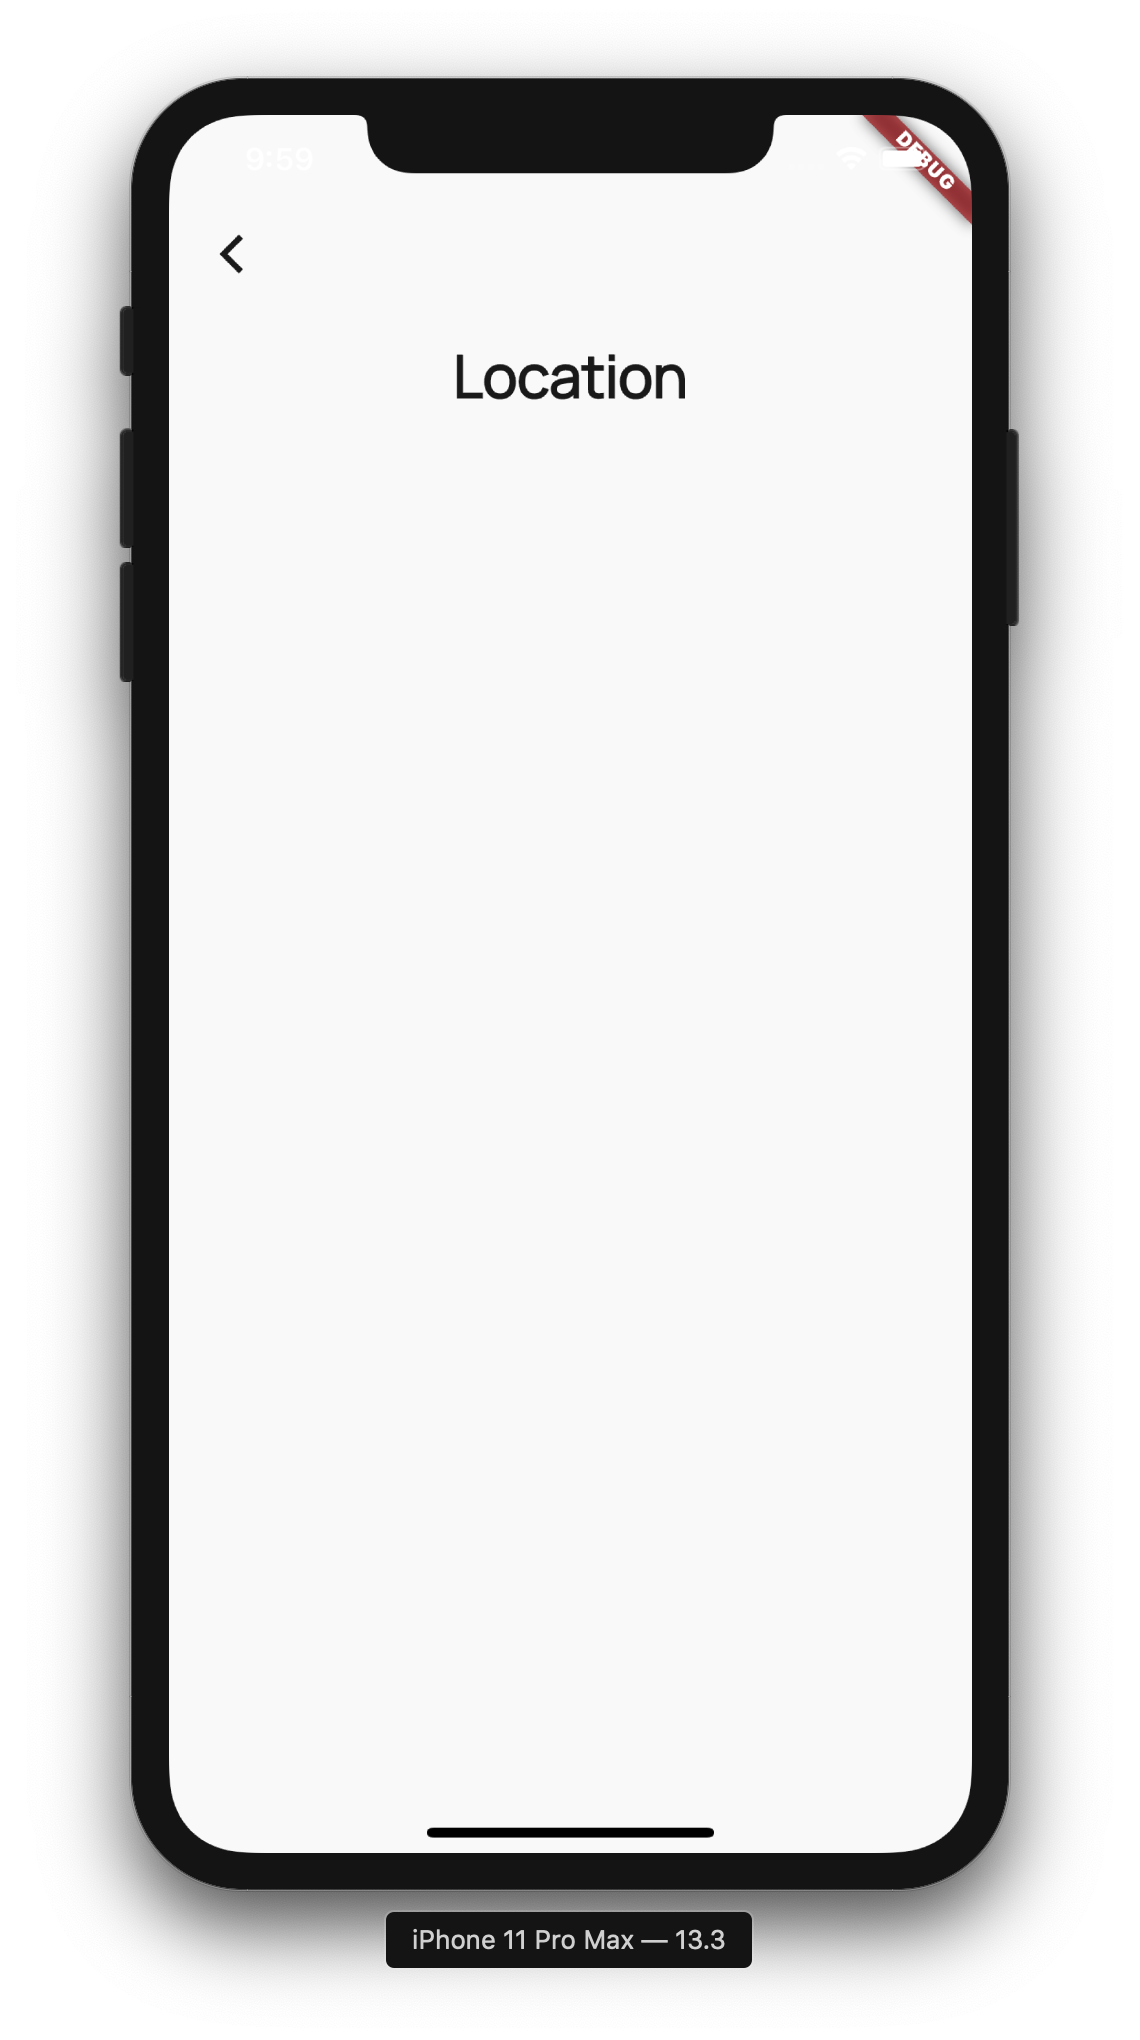
\includegraphics[scale=0.25]{location_detail}
	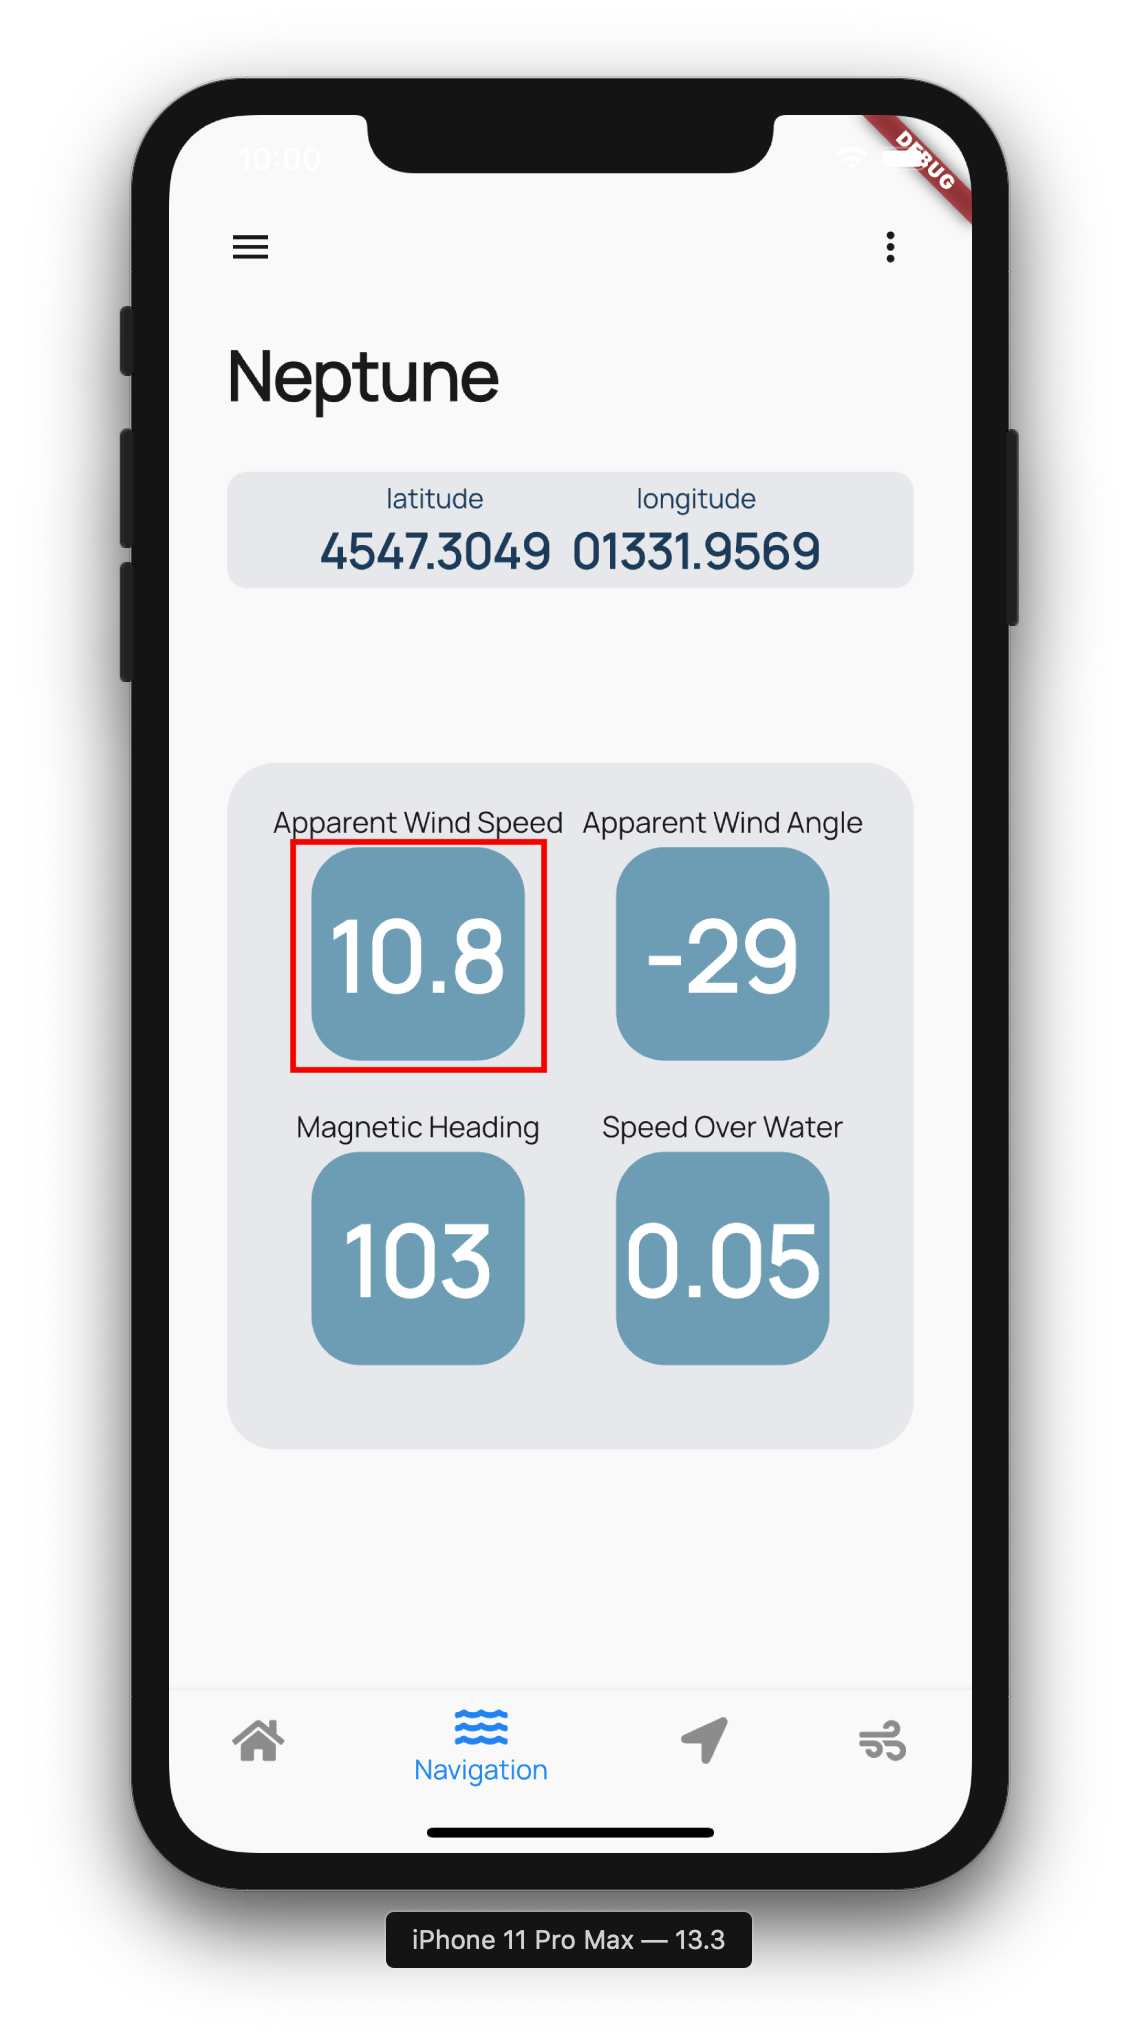
\includegraphics[scale=0.25]{navigation_tap}
	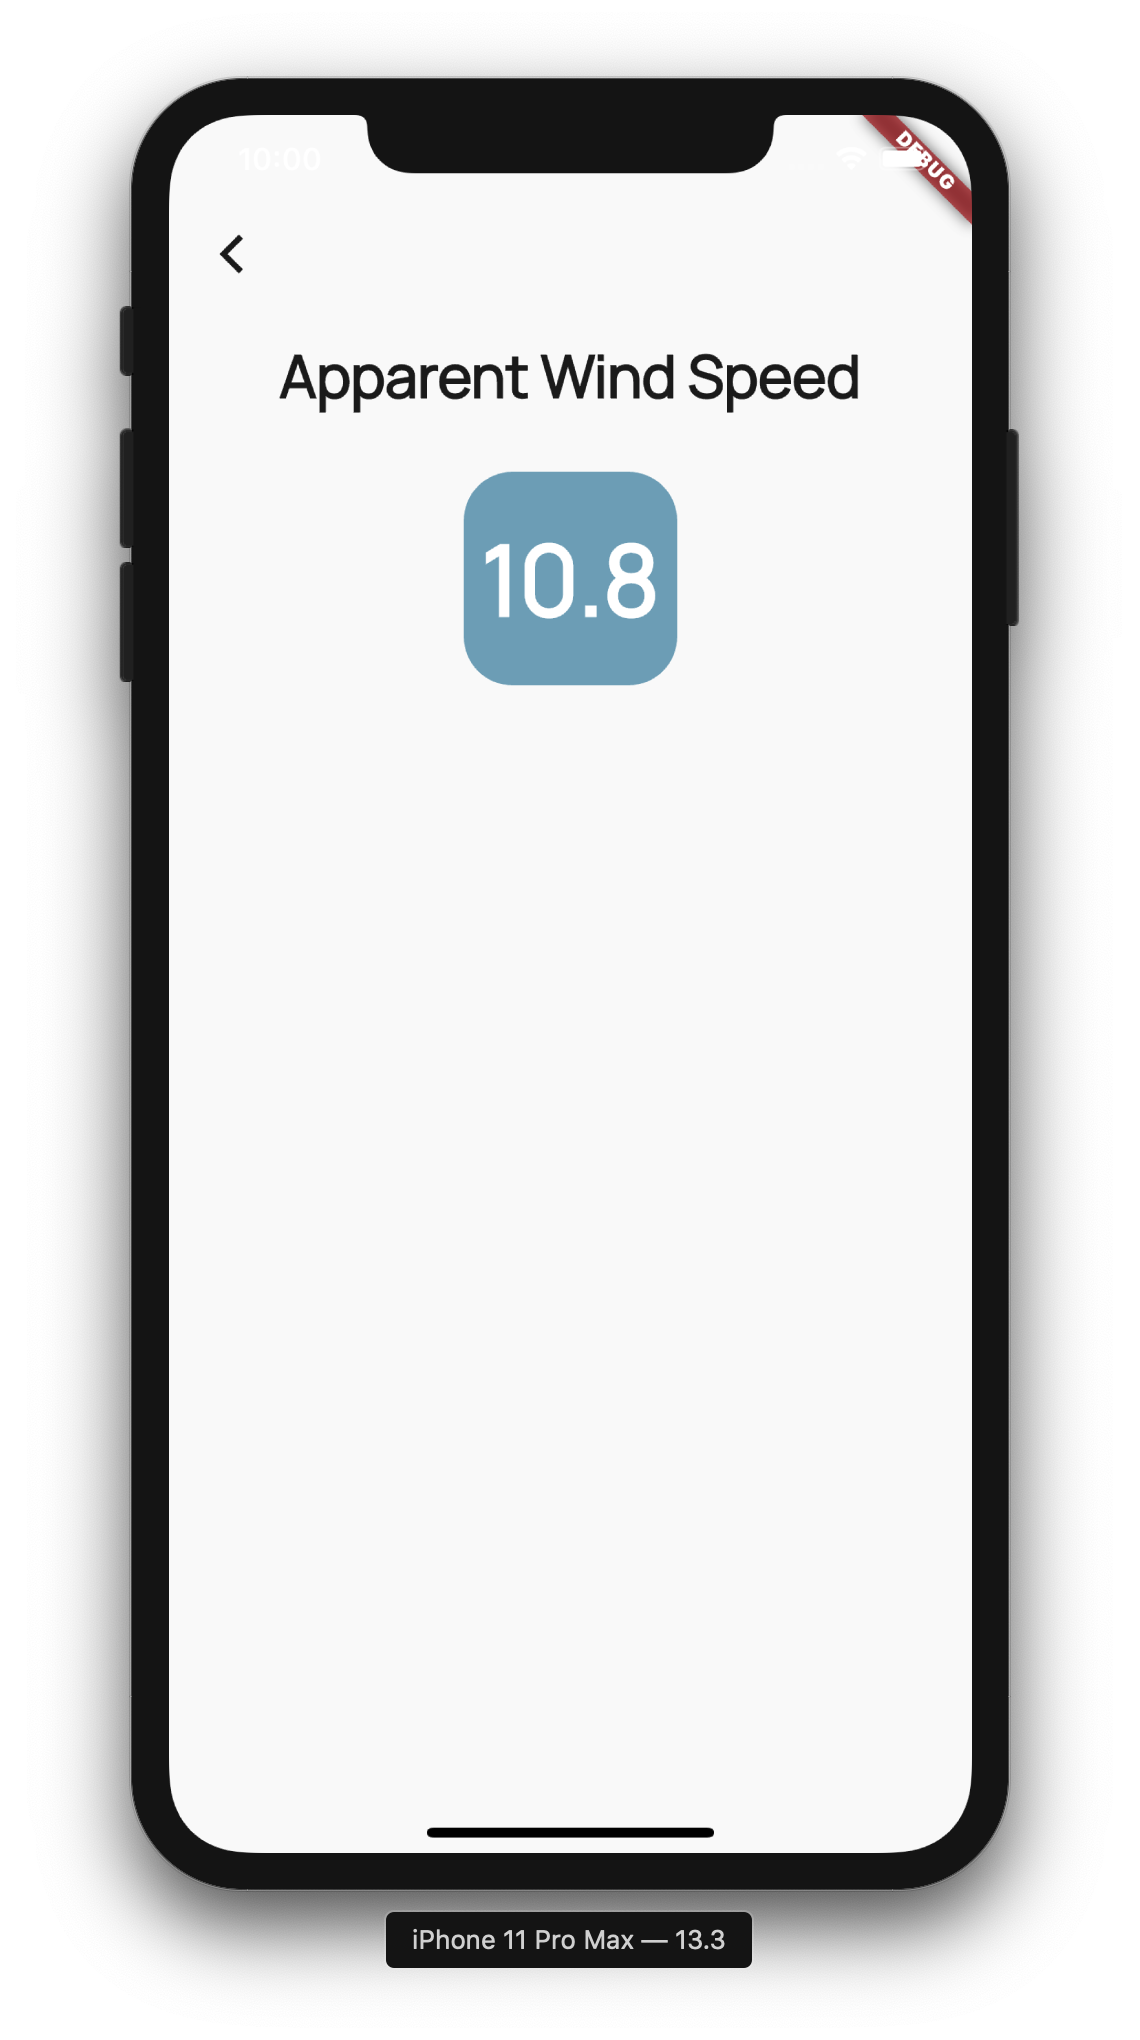
\includegraphics[scale=0.25]{navigation_detail}
	\caption[Sviluppi futuri - Location e Navigation]{Analogamente per la schermata \textit{Dashboard}, lo stesso avviene sia per il Widget \textit{Location}, sia per la schermata \textit{Navigation} (facendo tap sul dato \textit{Apparent Wind Speed})}\label{xyz}
\end{figure}

\subsection{Grafici e schermate dedicate ai dati}
Una funzionalità molto importante che aiuterebbe l'equipaggio nelle varie decisioni è la realizzazione di una pagina dedicata alla descrizione del dato. Questa funzionalità è stata in parte implementata, ovvero, è già stato predisposto il meccanismo per rilevare l'evento del tocco su un determinato dato e l'apertura della corrispondente schermata. Come si può vedere dagli screenshot, nella fase finale dell'applicazione le schermate sono vuote. Questa funzionalità è già stata predisposta per le schermate \textit{Dashboard}, \textit{Navigation} e per il Widget \textit{Location}. In queste schermate potrebbero essere illustrate delle descrizioni specifiche del dato ed eventualmente uno storico degli eventi riguardo a tale dato. In particolare, per \textit{eventi} si vuole intendere il verificarsi di una forte variazione del valore di un determinato dato, in cui tale variazione risulta essere anomala e può quindi essere motivo di attenzione.

Nella medesima schermata potrebbe essere aggiunto un grafico che illustra tutte le variazioni del dato nel tempo. Il vantaggio di utilizzare questo strumento, permette all'utente di visualizzare in maniera immediata se vi sono state delle variazioni anomale. I grafici possono sfruttare la \textit{cache} che è stata implementata nel \textit{Repository} dell'app. In questo modo, il grafico può attingere i dati da tale fonte.

\subsection{Aggiunta di componenti grafiche}
Per facilitare la fruizione delle informazioni proposte dall'applicazione, sarebbe utile l'implementazione di alcuni componenti grafici dedicati. Ad esempio, potrebbe essere realizzata una \textit{bussola}, con l'utilizzo del giroscopio e dell'accelerometro. La bussola può essere utilizzata per rendersi conto della direzione attuale verso la quale la barca si sta dirigendo.

\subsection{Introduzione di nuovi temi}
L'applicazione così realizzata permette di avere soltanto due temi: \textit{default} e ad \textit{alto contrasto}. Per come è stata strutturata l'applicazione è possibile supportare soltanto due temi. Con delle piccole variazioni al codice, è possibile gestire più temi, in modo che l'utente possa scegliere opportunatamente quello che ritiene più adatto alla situazione in cui si trova.

\subsection{Autenticazione degli utenti}
Aggiungere un servizio di autenticazione degli utenti potrebbe essere utile per capire quali membri della squadra o del team tecnico accedono ai dati e a quali dati. In questo modo è possibile creare un servizio che sia più completo anche dal punto di vista della sicurezza.

\section{Considerazioni sull'approccio cross-platform}
Negli ultimi anni, sempre più aziende cominciano a considerare l'approccio cross-platform come il più conveniente secondo diversi punti di vista. Come è già stato esplicitato durante la tesi, questo approccio è un ottimo compromesso tra \textit{performance}, in quanto questi framework interagiscono nativamente con la componentistica del dispositivo (in particolare con i sensori), e \textit{risorse economiche}. Lo sviluppo di un'applicazione con un framework cross-platform riduce i costi in quanto non è necessario assumere sviluppatori che la realizzino per ogni singola piattaforma e permette all'azienda di affrontare meglio il \textit{time-to-market}. Inoltre vi è un solo codice sorgente che viene gestito da un unico team di sviluppo.

Aziende molto importanti a livello mondiale si sono decise di utilizzare un framework cross-platofrom. In particolare, le aziende che verranno citate hanno sviluppato la loro applicazione utilizzando Flutter \cite{flutter_showcase}:
\begin{enumerate}
	\item \textbf{Alibaba}: uno dei più grandi e-commerce al mondo con milioni di utenti, ha realizzato la sua applicazione mobile per poter acquistare i prodotti offerti;
	\item \textbf{Tencent}: questa azienda ha utilizzato Flutter su molteplici applicazioni. L'azienda fornisce principalmente servizi di intrattenimento (gaming) e di comunicazione (telefonia e messaggistica);
	\item \textbf{New York Times}: ha realizzato un gioco disponibile per Android, iOS, Windows e macOS.
\end{enumerate}

L'aumento dello sviluppo di applicazioni cross-platform è dato principalmente dall'evoluzione tecnologica verificatesi negli ultimi anni: prima i software multipiattaforma non garantivano delle prestazioni e dei risultati paragonabili alle corrispondenti applicazioni native.

\section{Considerazioni su Dart}
Dart è un linguaggio ben strutturato e che si è rivelato flessibile ed efficiente. Personalmente, sono convinto che il successo del linguaggio sia dato proprio dall'esperienza accumulata negli anni da Google, la quale affonda le proprie radici nello sviluppo Web. È un linguaggio che può sostituire JavaScript, sia lato client e sia lato server. A causa della scarsa diffusione, nei primi anni Dart rimase nel buio. Grazie all'avvento di Flutter, gli sviluppatori stanno scoprendo le potenzialità di questo linguaggio, aumentate durante gli anni.

Ho trovato Dart un linguaggio molto flessibile grazie ai molteplici paradigmi che supporta. È molto apprezzabile la vicinanza della sua sintassi a linguaggi come Java e JavaScript, facilitando l'apprendimento del linguaggio. Il linguaggio contiene delle caratteristiche particolari che mi hanno permesso di implementare delle soluzioni eleganti a fronte di determinate problematiche.
Ho particolarmente apprezzato il doppio approccio alla compilazione \textit{AOT} e \textit{JIT}, che permette l’individuazione di errori già in fase di compilazione, riducendo notevolmente il tempo dedicato al \textit{debugging}, senza però privare il linguaggio delle astrazioni che si basano sulla tipizzazione a tempo di esecuzione del codice.

Essendo un Android developer, ho potuto notare le differenze rispetto a \textit{Kotlin}. Dart risulta essere un linguaggio molto più pulito rispetto a Kotlin anche se entrambi hanno di fatto sintassi molto simile e meccanismi comuni, come la tipizzazione \textit{implicita} ed \textit{esplicita}.

Sulla base della mia esperienza sostengo che Google abbia scelto Dart come linguaggio per la realizzazione di applicazioni in Flutter perchè l'azienda aveva già sviluppato delle librerie Web per tale linguaggio, come ad esempio la libreria \textit{Material}. Di conseguenza, risultava più facile realizzare applicazioni in Flutter mediante Dart. Se avessero deciso di utilizzare Kotlin come linguaggio per la scrittura di applicazioni in Flutter, il team di sviluppo avrebbe dovuto svolgere un lavoro ancora più oneroso.

Inoltre, sostengo che il punto a favore che aveva Dart rispetto a Kotlin era più di natura competitiva: Kotlin è un linguaggio nato nel 2011 e sviluppato da un'azienda della Repubblica Ceca, \textit{JetBrains}. Dart invece è stato realizzato direttamente da Google. Di conseguenza, sostengo che la scelta di Dart fosse stata presa anche per non far dipendere il destino del framework da un linguaggio sviluppato da un'azienda esterna a Google.

\section{Considerazioni su Flutter}
Nonostante la giovane età, Flutter sta diventando un punto di riferimento per lo sviluppo di applicazioni cross-platform. Sempre più aziende si avvicinano a questo framework come strumento di sviluppo. LinkedIn, secondo i dati di cui dispone, mostra come Flutter comincia ad essere una \textit{skill} molto richiesta agli sviluppatori in questo periodo e che la richiesta delle aziende a riguardo sta crescendo maggiormente rispetto a tutte le altre tecnologie mobile \cite{flutter_skill}. Un elemento da tenere in considerazione è l'enorme proliferazione di pacchetti e plugin su Pub. Questo significa che c'è un grande interesse attorno a questo framework e mostra anche come Flutter sia costantemente in evoluzione.

Dart si è rivelato essere un ottimo linguaggio per lo sviluppo di applicazioni cross-platform. Un linguaggio molto flessibile e completo in grado di risolvere le problematiche più spinose dello sviluppo mobile. Ritengo che in futuro, il mondo dello sviluppo di applicazioni mobili si polarizzerà principalmente in sostenitori di React Native e di Flutter. React Native e Flutter hanno due caratteristiche che li accomunano e che gli altri framework non possiedono: sono stati sviluppati da due aziende tecnologiche di livello mondiale (rispettivamente, Facebook e Google) e, come conseguenza di questo primo aspetto, hanno molti sviluppatori che sostengono e supportano il framework. Da quest'ultimo punto di vista Flutter è leggermente in svantaggio per il semplice fatto di essere approdato in questo mercato più tardi: sono convinto che nel giro di qualche anno riuscirà superare la metà degli sviluppatori che supporteranno React Native, in virtù anche del futuro sviluppo di Fuchsia.

Inoltre ho particolarmente apprezzato la metodologia utilizzata per realizzare le interfacce grafiche: il meccanismo della composizione dei Widget l'ho trovata affascinante dal punto di vista sia della scrittura ma anche della lettura del codice. Progettare la UI secondo questo approccio permette di produrre del codice molto pulito.

Considero molto positivo l'obiettivo a lungo termine avviato da Google, ovvero, quello di utilizzare Flutter come framework principale per lo sviluppo di applicazioni per \textit{qualsiasi} piattaforma, che questa sia Web, desktop, mobile o il futuro sistema operativo Fuchsia. È una visione molto ampia e di lungo termine che porterà i suoi benefici nei prossimi anni.

\section{Considerazioni personali}

\subsection{Scelta del framework}
Avendo un background come sviluppatore per applicazioni Android, ho particolarmente apprezzato questo framework sopratutto per queste caratteristiche:
\begin{enumerate}
	\item \textbf{Cross-platform}: ho sempre desiderato implementare applicazioni anche per i dispostivi iOS, ma non conoscendo Swift e nemmeno il sistema operativo, ho sempre declinato questa possibilità. Quando scoprii che Flutter era un framework che mi permetteva di realizzare applicazioni per entrambi i sistemi operativi ho subito avuto un forte interessamento ed ho cominciato nel giro di pochi giorni a sviluppare la prima applicazione, grazie anche alla conoscenza accumulata con Java;
	\item \textbf{Prestazioni}: essendo un framework multipiattaforma ho voluto accertarmi che l'applicazione prodotta rispettasse determinati parametri di efficienza e di performance. A seguito di alcuni test svolti sviluppando applicazioni che implementavano funzionalità diverse, ho avuto la possibilità di verificare tali requisiti;
	\item \textbf{Forte tipizzazione}: sviluppando applicazioni per Android, volevo continuare a sviluppare app utilizzando comunque un linguaggio fortemente tipizzato come Java, per poter continuare a trarre tutti i vantaggi dalla forte tipizzazione.
\end{enumerate}

Prima dell'avvento di Flutter ero già a conoscenza della presenza di React Native. Tuttavia, informandomi attraverso le esperienze di alcuni sviluppatori, non mi convinse come framework: alto consumo di memoria centrale, alto consumo di CPU, le prestazioni dell'applicazione non erano ottimali e non si avvicinavano a quelle di un'applicazione nativa. Inoltre, scrivere un'applicazione in React Native produce del codice molto verboso, a differenza di Flutter che produce del codice compatto. Altro aspetto che non mi ha convinto è la presenza del \textit{bridge} JavaScript per interagire con i moduli nativi del dispositivo, il quale rappresenta uno dei principali fattori che contribuisce al degrado complessivo delle prestazioni dell'applicazione.

La facilità nel realizzare delle interfacce grafiche è una ragione che mi ha convinto ancora di più ad adottare questo framework per lo sviluppo di app. Infatti è possibile realizzare UI complesse ma che siano comunque \textit{user-friendly}.

\subsection{Progettazione e sviluppo dell'applicazione}
L'esperienza di tirocinio svolta per lo sviluppo dell'applicazione è stata molto coinvolgente e ricca di spunti per la realizzazione di nuovi progetti in futuro. Mi ha permesso di ampliare le conoscenze riguardo il mondo cross-platform ed il mondo Flutter, permettendomi anche di far tesoro dell'esperienza accumulata durante lo sviluppo di questo progetto. Sono stato particolarmente affascinato dai pattern architetturali disponibili e sostengo che la mia scelta di implementare il pattern \textit{BLoC} sia stata una decisione corretta. È stata una scelta ben ponderata, in quanto volevo costruire una struttura sufficientemente stabile, ma allo stesso tempo, flessibile per poter supportare le funzionalità future che verranno implementate nell'applicazione.

Sono molto soddisfatto di aver fatto esperienza anche nella realizzazione dell'interfaccia grafica, un aspetto un po' carente nel mio bagaglio.

La soddisfazione più grande rimane il fatto di aver realizzato un'applicazione che può essere distribuita sia per Android che per iOS, a partire da un unico codice sorgente. È un risultato che mi rende molto felice e che mi ha particolarmente sorpreso ed entusiasmato. 

Complessivamente, il processo di sviluppo mi ha invogliato molto a superare determinati limiti personali e ad andare oltre a quella \textit{zona di comfort}, per esplorare e apprendere nuove conoscenze. Ritengo che esperienze come questa, debbano essere svolte il più possibile, in quanto permettono alla persona di crescere in modo esponenziale sotto diversi aspetti contemporaneamente: a partire dall'organizzazione del progetto, all'organizzazione dei tempi, delle risorse, all'analisi dei requisiti. Aspetti che vanno ad unire quelle che vengono definite \textit{hard skills} e \textit{soft skills}, entrambe di fondamentale importanza nel mondo dell'innovazione.